\section{EVALUATION}
\label{ch:evaluation}

%\noindent 為了驗證本研究方法的可行性，我們提出以下 Research Questions (RQs):
\noindent To verify the feasibility of our research methodology, the following Research Questions (RQs) are proposed:

\begin{itemize}
    \item \textbf{RQ1: Can KOFTA find options or optional arguments that are not documented ?} %KOFTA 是否能夠找到未紀錄於文檔中的選項或選項參數？
    \item \textbf{RQ2: Does a multi-argument forkserver truly reduce the overhead of multi-parameter fuzzing ?} %多參數 forkserver 是否真的能夠減少多參數模糊測試的額外開銷
\iffalse
    \item \textbf{RQ3：KOFTA 是否能有與 Wei-fuzz 相當的測試效果？}
    \item \textbf{RQ4：KOFTA 是否能夠幫助 Wei-fuzz 達到更高的測試覆蓋率？}
\fi
\end{itemize}

%\noindent 所有實驗皆在以下的環境中進行：
All experiments were conducted in the following environment:
\iffalse
\begin{itemize}
    \item Ubuntu 20.04.6 LTS
    \item 32 Cores CPU
    \item 128G Memory
\end{itemize}
\else
\texttt{Ubuntu 20.04.6 LTS}, \texttt{32 Cores CPU}, and \texttt{128G Memory}.
\fi
%\noindent 實驗的初始種子皆為 AFL 提供的預設種子。目標程式的版本如表（Table \ref{tab:targets}）所示。
And, \texttt{initial seeds} for all experiments were default seeds in AFL. The \texttt{versions of the target programs} are shown in the table (Table \ref{tab:targets}).

\begin{table}[h!]
    \centering
    \begin{threeparttable}
        \caption{Target Programs} %目標程式
        \label{tab:targets}
        \begin{tabular}{>{\ttfamily}c|>{\ttfamily}c|>{\ttfamily}c}
            \toprule
            \textbf{Project} & \textbf{Program} & \textbf{Version} \\
            \midrule
            Binutils & objdump & 2.44\\
            Binutils & objcopy & 2.44\\
            Binutils & readelf & 2.44\\
            Libxml2 & readelf & 2.14.4\\
            Libtiff & tiffcp & 4.7.0\\
            Libtiff & tiffcrop & 4.7.0\\
            MuPDF & mutool & 1.26.3\\
            Giflib & giftool & 5.2.2\\
            Libsixel & img2sixel & 1.10.5\\
            \bottomrule
        \end{tabular}
    \end{threeparttable}
\end{table}

\subsection{RQ1}

%與過去多參數模糊測試的研究相比，KOFTA 除了無須借助人力，另一個主要差別在於分析的「對象」。
Compared to past research on multi-argument fuzzing, KOFTA differs not only in that it eliminates the need for human intervention, but also in the "object" of analysis.

%其他研究使用目標程式「使用手冊（\texttt{man} 指令）」或「\texttt{--help} 選項」的內容作為分析選項、選項參數的依據；

%KOFTA 分析的是「原始碼」、「執行階段的動態回饋」。這種方式產生的選項、選項參數更能符合實際的情況。
KOFTA analyzes "source code" and "dynamic feedback during execution." This approach generates options and optional arguments that better reflect real-world scenarios.

%尤其是當使用手冊等文檔「記載不周」、「資訊過時」，產生的選項也會是錯誤或缺漏的。

%因此，RQ：「KOFTA 是否能夠找到未紀錄於文檔中的選項或選項參數」被提出。
%Therefore, RQ "Can KOFTA find options or optional arguments that are not documented?" was raised.

%我們統計了 KOFTA 在 16 個小時內使用過的選項、選項參數，並與「使用手冊（\texttt{man} 指令）」或「\texttt{--help} 選項」的內容相比，結果呈現於表格（Table \ref{tab:ud-opt-arg}）中。可以發現，KOFTA 透過靜態分析能夠找到所有記載於文檔中的選項，並從 \texttt{objcopy}、\texttt{readelf}、\texttt{tiffcp} 的原始碼中找到未記載的選項。污染源推論的效果更加顯著，可以從四個目標程式中找到 37 個未記載的選項參數。
We analyzed the options and optional arguments used by KOFTA over a 16-hour period and compared them with the contents of the "User Manual (\texttt{man} command)" or "\texttt{--help}" options. The results are presented in a table (Table \ref{tab:ud-opt-arg}). It can be seen that KOFTA, through static analysis, can find all options in the documentation and also find undocumented options in the source code of \texttt{objcopy}, \texttt{readelf}, and \texttt{tiffcp}. The effect of taint inference is even more significant, finding 37 undocumented optional arguments from four target programs.

%\vfill

\begin{table}[h!] %[hb]
    \centering
    \begin{threeparttable}
        \caption{\footnotesize Undocumented Options and Option Arguments} %未紀錄於文檔中的選項及選項參數數量
        \label{tab:ud-opt-arg}
        \begin{tabularx}{0.48\textwidth}{
                >{\ttfamily}c|
                >{\ttfamily\centering\arraybackslash}X
                >{\ttfamily\centering\arraybackslash}X
                >{\ttfamily\centering\arraybackslash}X
                >{\ttfamily\centering\arraybackslash}X}
            \toprule
            \textbf{Program}  & \textbf{\#Doc.Opt.} & \textbf{Comp.} & \textbf{\#UD.Opt.} & \textbf{\#UD.Optarg.}\\
            \midrule
            objdump  & 67 & \checkmark & 0 &  1\\
            objcopy  & 99 & \checkmark & 3 & 18\\
            readelf  & 48 & \checkmark & 3 &  0\\
            xmllint  & 64 & \checkmark & 0 &  0\\
            tiffcp   & 20 & \checkmark & 1 &  4\\
            tiffcrop & 38 & \checkmark & 0 & 14\\
            \midrule
            total    & 336 & \checkmark & 7 & 37\\
            \bottomrule
        \end{tabularx}
        \begin{tablenotes}
            \small
            \item Doc. = Documented ; UD. = Undocumented
            \item Opt. = Options ; Optarg. = Optional Arguments
            \item Comp. = KOFTA whether to find all documented options completely.
        \end{tablenotes}
    \end{threeparttable}
\end{table}

\iffalse

\subsubsection{Case Study: \texttt{readelf}}
\label{subsec:rq1-case-readelf}

KOFTA 總共在 \texttt{readelf} 的原始碼中發現了三個未記載於文件中的選項：\texttt{-i}、 \texttt{-N} 與 \texttt{--dwarf-check}。參考節錄的 readelf 命令列參數解析程式碼片段（Listing \ref{lst:readelf-udopt}），選項「\texttt{-i}」會以「\texttt{DISASS\_DUMP}」作為參數呼叫 \texttt{request\_dump()}；選項「\texttt{-i}」與「\texttt{-N}」則分別會影響「\texttt{do\_section\_details}」與「\texttt{dwarf\_check}」兩個旗標變數（flag）。以上操作都無法使用其他選項組合達成、取代，因此 KOFTA 可以探索其他基於文件的模糊測試工具無法到達的地方。

%解析未記載於文檔的選項
\begin{lstlisting}[float=h!, caption=\texttt{readelf}: Parse Undocumented Option, label=lst:readelf-udopt]
switch (c)
{
  case 'i':
    request_dump (dumpdata, DISASS_DUMP);
    break;
  case 'N':
    do_sections = true;
    do_section_details = true;
    break;
  case OPTION_DWARF_CHECK:
    dwarf_check = true;
    break;
}
\end{lstlisting}
%\vfill

\subsubsection{Case Study: \texttt{tiffcrop}}

KOFTA 總共在 \texttt{tiffcrop} 的執行過程中發現了 14 個未記載於文件中的選項參數（Table \ref{tab:tiffcrop-udoptarg}），它們皆是選項「\texttt{-P}」的選項參數。根據 \texttt{tiffcrop} 的使用手冊描述，該選項參數代表一種紙張的大小（例如 a4 代表 8.27x11.69 英吋），程式會調整輸出的圖片以符合該紙張的尺寸；但並未列舉可以使用的選項參數，反而進一步地說明可以使用「\texttt{-P list}」列出所有支援的選項參數。這種需要額外步驟才能確認選項參數的方式，大大增加了人工分析的成本，對於那些使用自然語言處理、人工智慧等方式分析手冊的研究來說，要產生這類選項參數更是困難重重。

\begin{table}[h!] %[hb]
    \centering
    \caption{\texttt{tiffcrop}: Undocumented Option Arguments} %未記載於文檔的選項參數
    \label{tab:tiffcrop-udoptarg}
    \begin{tabularx}{0.45\textwidth} {
        | >{\ttfamily\centering\arraybackslash}X
        | >{\ttfamily\centering\arraybackslash}X
        | >{\ttfamily\centering\arraybackslash}X | }
        \hline
        a10 & a7 & a8\\
        \hline
        c3 & default & dsheet\\
        \hline
        executive & half-letter & ledger\\
        \hline
        legal & letter & list\\
        \hline
        superb & tabloid & \\
        \hline
    \end{tabularx}
\end{table}
\fi

\iffalse
\subsection{RQ3}
\label{sec:rq-eff}

即使 KOFTA 能夠省下許多人工成本，甚至能夠發現未記載於文件中的選項、選項參數，幫助模糊測試探索更廣泛的輸入空間；但是這些好處也伴隨著由污染源推論產生的額外開銷。為了評估污染源推論所帶來的利弊，我們以 Wei-fuzz 為主要的比較對象，並提出RQ:「KOFTA 是否能有與 Wei-fuzz 相當的測試效果」？

我們統計並比較了 KOFTA 與 Wei-fu」zz 測試總共 6 個目標程式在 16 個小時內的表現。為了避免隨機性影響結果，對於每個目標程式都會進行 4 輪的測試並計算平均路徑覆蓋率。從結果（Figure \ref{fig:kofta-vs-wei}）可以看出，6 個目標程式中正好有一半贏過 Wei-fuzz 的表現。進一步將結果整理成表格（Table \ref{tab:kofta-vs-wei}）後，雖然可以知道 KOFTA 整體平均路徑覆蓋率低於 Wei-fuzz 約 2\% 左右，但 KOFTA 還有能夠省下人工成本這個優點。同時能夠發現 KOFTA 對於特定的目標程式有明顯的喜好，測試結果最差的 \texttt{xmllint} 平均輸了 43\%；而最好的 \texttt{objcopy} 贏了高達 39\% 。

為了了解是什麼原因造成 KOFTA 對於目標程式的喜好差異，我們將每個目標程式中選項的數量、選項參數必要性為「必要」或「非必要」的比例、模糊測試探索發現的選項參數數量進行統計（Table \ref{tab:kofta-preference-1}），可以發現表現最差的 \texttt{xmllint} 同時有著最低的「必要性比例」與最低的「選項參數探索數量」；而表現最好的 \texttt{objcopy} 則擁有第二高的「必要性比例」與最高的「選項參數探索數量」。這個看似直觀的結論，目前似乎仍然無法很好地解釋 \texttt{objdump} 與  \texttt{readelf} 等等其他目標程式的結果。應該還存在著其他的因素，影響了 KOFTA 對其的喜好。

%\vfill

\begin{table}[H] %[hb]
    \centering
    \begin{threeparttable}
        \caption{KOFTA v.s. Wei-fuzz}
        \label{tab:kofta-vs-wei}
        \begin{tabularx}{0.5\textwidth}{
                >{\ttfamily}c|
                >{\ttfamily\centering\arraybackslash}X
                >{\ttfamily\centering\arraybackslash}X
                >{\ttfamily\centering\arraybackslash}X}
            \toprule
            \textbf{Program}  & \textbf{KOFTA\textsuperscript{*}} & \textbf{Wei-fuzz\textsuperscript{*}} & \textbf{\%} \\
            \midrule
            objdump  &  9879 & 12531 & -21.17\% \\
            objcopy  &  8084 &  5814 & \textbf{+39.05\%} \\
            readelf  & 30788 & 25367 & +21.37\% \\
            xmllint  &  6214 & 10961 & \textbf{-43.31\%} \\
            tiffcp   &  7219 &  9415 & -23.32\% \\
            tiffcrop &  8151 &  7726 & +5.50\% \\
            \midrule
            total    & 11722 & 11969 & -2.06\% \\
            \bottomrule
        \end{tabularx}
        \begin{tablenotes}
            \small
            \item \texttt{\textsuperscript{*}} = Average Paths Found
        \end{tablenotes}
    \end{threeparttable}
\end{table}

%\vfill

\begin{table}[H] %[hb]
    \centering
    \begin{threeparttable}
        \caption{影響 KOFTA 對於目標程式喜好的因素（一）}
        \label{tab:kofta-preference-1}
        \begin{tabularx}{0.5\textwidth}{
                >{\ttfamily}c|
                >{\ttfamily\centering\arraybackslash}X
                >{\ttfamily\centering\arraybackslash}X
                >{\ttfamily\centering\arraybackslash}X
                >{\ttfamily\centering\arraybackslash}X}
            \toprule
            \textbf{Program}  & \textbf{\%} & \textbf{\#Opt.} & \textbf{\%HasOptarg} & \textbf{\#FuzzOptarg} \\
            \midrule
            objdump  &  -21.17\%          &  67 & 38.81\%          & 352 \\
            objcopy  &  \textbf{+39.05\%} & 102 & 67.73\%          & \textbf{685} \\
            readelf  &  +21.37\%          &  51 & 31.37\%          &  79 \\
            xmllint  &  \textbf{-43.31\%} & 156 & \textbf{16.03}\% & \textbf{7} \\
            tiffcp   &  -23.32\%          &  21 & 47.62\%          & 131 \\
            tiffcrop &   +5.50\%          &  38 & \textbf{73.68\%} & 284 \\
            \bottomrule
        \end{tabularx}
        \begin{tablenotes}
            \small
            \item Opt. = Options
            \item HasOptarg = 必要性「必要」或「非必要」的選項參數
            \item FuzzOptarg = 由污染源推論發現的選項參數
        \end{tablenotes}
    \end{threeparttable}
\end{table}

%\newpage

%\null\vfill
\begin{figure}[H] %[h!]
    \centering
    \begin{subfigure}[]{0.45\textwidth}
        \centering
        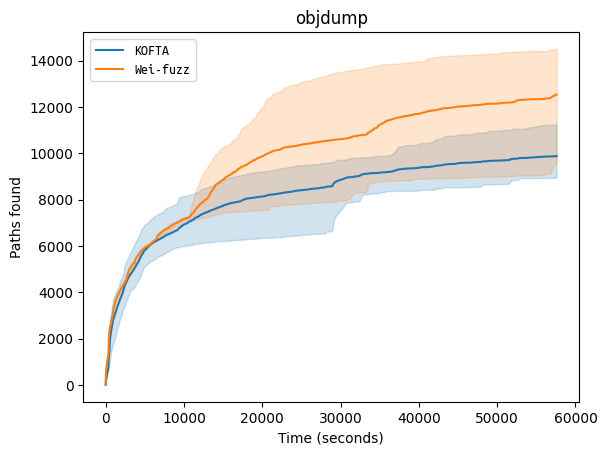
\includegraphics[width=0.8\textwidth]{img/16h/objdump-16h.png}
    \end{subfigure}
    \begin{subfigure}[]{0.45\textwidth}
        \centering
        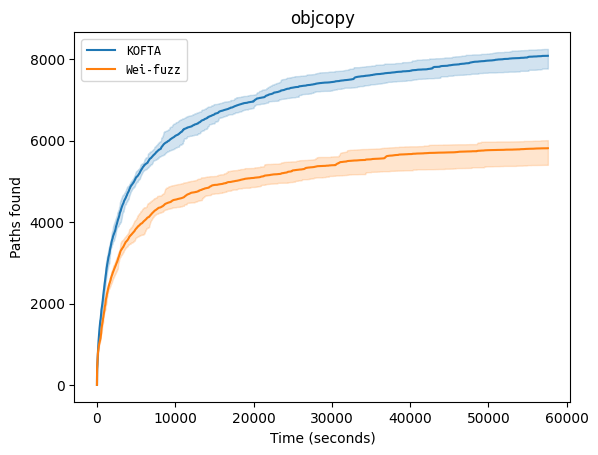
\includegraphics[width=0.8\textwidth]{img/16h/objcopy-16h.png}
    \end{subfigure}

\end{figure}

\begin{figure}[H] %[h!]
    \centering
    \begin{subfigure}[]{0.45\textwidth}
        \centering
        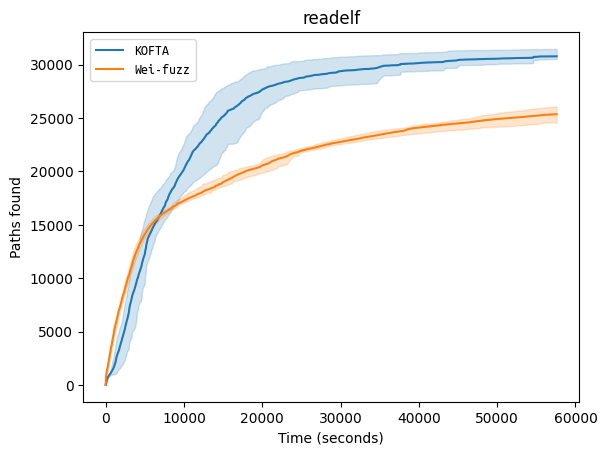
\includegraphics[width=0.8\textwidth]{img/16h/readelf-16h.png}
    \end{subfigure}
    \begin{subfigure}[]{0.45\textwidth}
        \centering
        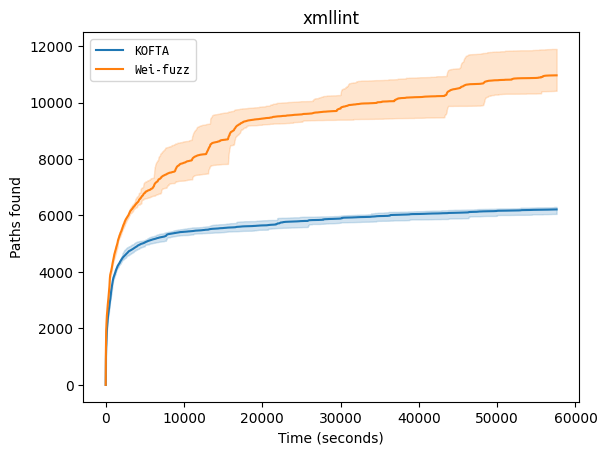
\includegraphics[width=0.8\textwidth]{img/16h/xmllint-16h.png}
    \end{subfigure}

\end{figure}

\begin{figure}[H] %[h!]
    \centering
    \begin{subfigure}[]{0.45\textwidth}
        \centering
        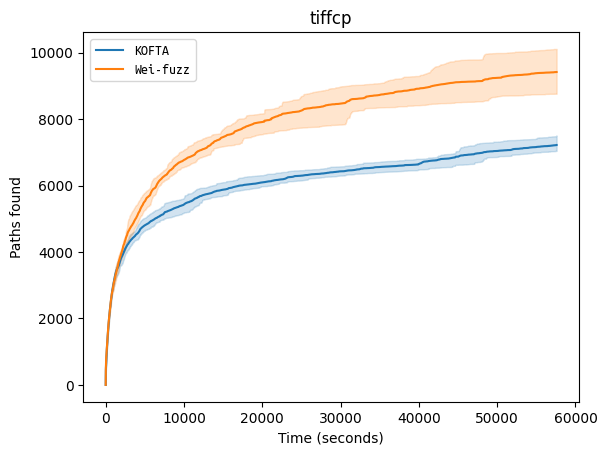
\includegraphics[width=0.8\textwidth]{img/16h/tiffcp-16h.png}
    \end{subfigure}
    \begin{subfigure}[]{0.45\textwidth}
        \centering
        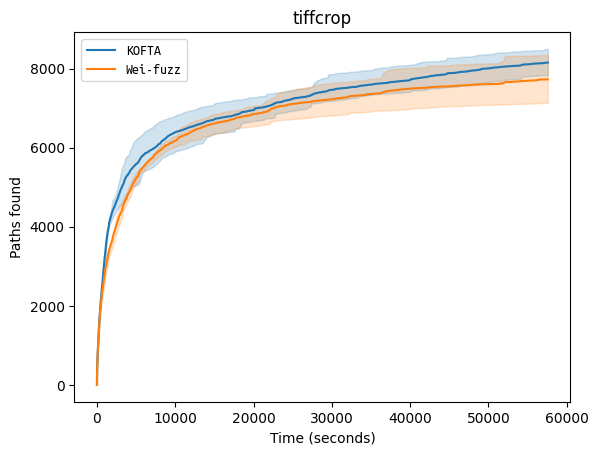
\includegraphics[width=0.8\textwidth]{img/16h/tiffcrop-16h.png}
    \end{subfigure}
    \caption{KOFTA v.s. Wei-fuzz}
    \label{fig:kofta-vs-wei}
\end{figure}

\iffalse
\begin{figure}[H] %[h!]
    \centering
    \begin{subfigure}[]{0.45\textwidth}
        \centering
        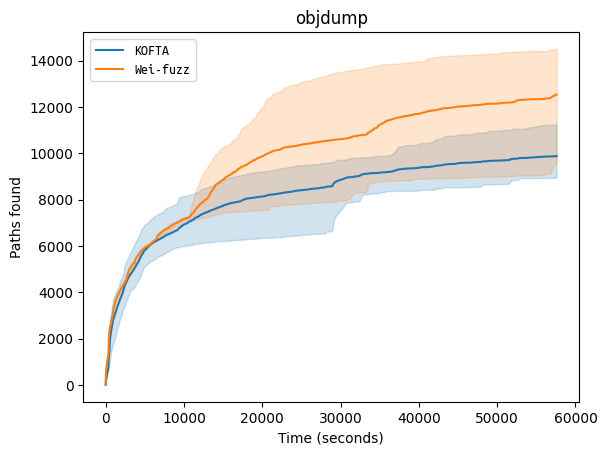
\includegraphics[width=0.8\textwidth]{img/16h/objdump-16h.png}
    \end{subfigure}
    \begin{subfigure}[]{0.45\textwidth}
        \centering
        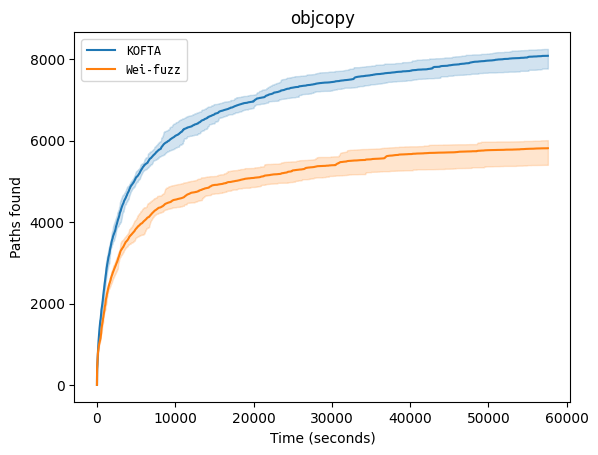
\includegraphics[width=0.8\textwidth]{img/16h/objcopy-16h.png}
    \end{subfigure}
    \begin{subfigure}[]{0.45\textwidth}
        \centering
        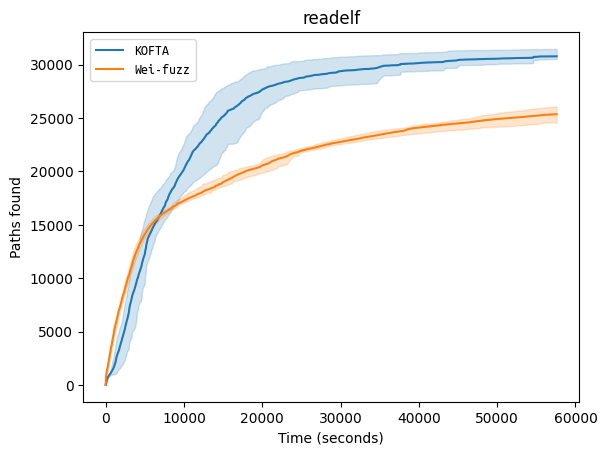
\includegraphics[width=0.8\textwidth]{img/16h/readelf-16h.png}
    \end{subfigure}
    \begin{subfigure}[]{0.45\textwidth}
        \centering
        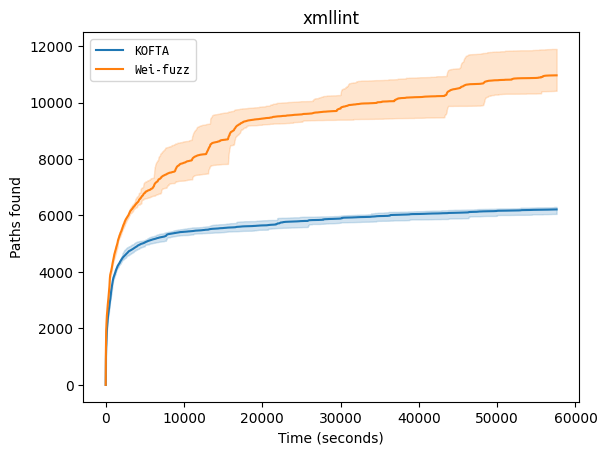
\includegraphics[width=0.8\textwidth]{img/16h/xmllint-16h.png}
    \end{subfigure}
    \begin{subfigure}[]{0.45\textwidth}
        \centering
        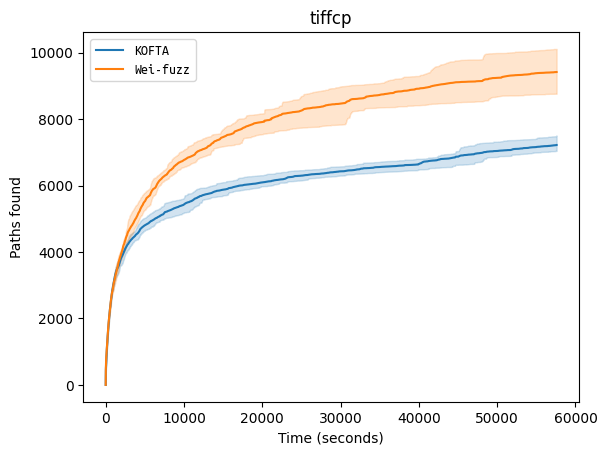
\includegraphics[width=0.8\textwidth]{img/16h/tiffcp-16h.png}
    \end{subfigure}
    \begin{subfigure}[]{0.45\textwidth}
        \centering
        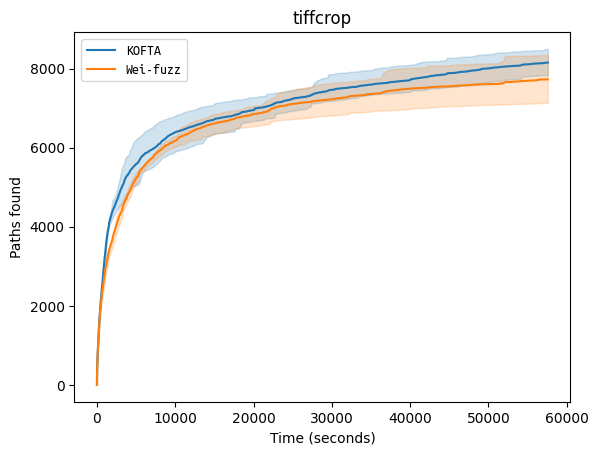
\includegraphics[width=0.8\textwidth]{img/16h/tiffcrop-16h.png}
    \end{subfigure}
    \caption{KOFTA v.s. Wei-fuzz}
    \label{fig:kofta-vs-wei}
\end{figure}
\fi

%\vfill\null

%\newpage

\subsection{RQ4}
\label{sec:rq-cov}

KOFTA 依據目標程式執行階段回饋的提示生成選項參數，和單純參考使用手冊等文件寫死的選項參數相比，或許能夠更符合實際測試使用上的需要。換句話說，動態生成的選項參數或許能和測試時使用的輸入檔產生更好的配合，適時地探索不同的路徑、提高覆蓋率。為了驗證這個推論，我們將蒐集 KOFTA 測試時發現的選項參數、提供給 Wei-fuzz 進行測試，並提出RQ:「KOFTA 是否能夠幫助 Wei-fuzz 達到更高的測試覆蓋率」？

這個實驗將分成兩個階段：選項參數蒐集階段、比較 Wei-fuzz 階段。首先在選項參數蒐集階段我們會使用 KOFTA 與其變體 KOFTA-nd 進行測試。變體 KOFTA-nd 為 KOFTA 停用所有文件變異（havoc stage、splicing stage）的版本，也就是初始種子將不會進行變異並全程作為測試輸入檔使用。模糊測試皆持續 1 小時，並將這段時間中找到的選項、選項參數整理成 Wei-fuzz 使用的參數組態檔格式。

在下個階段中，我們讓 Wei-fuzz 使用預設的參數組態檔與 KOFTA 生成的參數組態檔進行測試比較。為了避免隨機性影響結果，各個目標搭配參數組態檔共會進行 4 輪測試並計算平均路徑覆蓋率。每輪測試皆為 1 個小時，目的是要觀察短時間內 KOFTA 產生的選項參數是否有幫助。因為要驗證的是選項參數與輸入檔是否配合，而測試時間越長文件變異的次數也就越多，隨機變異後的文件不是主要的觀察目標，所以我們將實驗時間縮短，觀察那些只經過些微變化後的輸入檔與選項參數搭配的效果。

從實驗結果的圖表（Figure \ref{fig:kofta-conf-vs-wei-conf}）可以知道 KOFTA 產生的參數設定檔在 6 個目標中有 4 個產生了更高的路徑覆蓋率。將結果製作成表格（Table \ref{tab:kofta-vs-wei-conf}）觀察，發現測試結果最差的 \texttt{xmllint} 平均輸了 34\%；而最好的 \texttt{readelf} 贏了高達 16\% 。整體而言，使用 KOFTA 產生的參數組態檔可以幫助 Wei-fuzz 多產生約 1.85\% 的路徑覆蓋率。

%\vfill

\begin{table}[h!] %[ht]
    \centering
    \begin{threeparttable}
        \caption{KOFTA 選項參數 v.s. Wei-fuzz 選項參數}
        \label{tab:kofta-vs-wei-conf}
        \begin{tabularx}{0.5\textwidth}{
                >{\ttfamily}c|
                >{\ttfamily\centering\arraybackslash}X
                >{\ttfamily\centering\arraybackslash}X
                >{\ttfamily\centering\arraybackslash}X}
            \toprule
            \textbf{Program}  & \textbf{KOFTA\textsuperscript{*}} & \textbf{Wei-fuzz\textsuperscript{*}} & \textbf{\%} \\
            \midrule
            objdump  &  5498 &  5264 &  +4.43\% \\
            objcopy  &  3682 &  3479 &  +5.83\% \\
            readelf  & 13809 & 11849 & \textbf{+16.54}\% \\
            xmllint  &  4402 &  6310 & \textbf{-30.24}\% \\
            tiffcp   &  4607 &  4911 &  -6.20\% \\
            tiffcrop &  5140 &  4648 & +10.58\% \\
            \midrule
            total    &  6189 &  6077 &  +1.85\% \\
            \bottomrule
        \end{tabularx}
        \begin{tablenotes}
            \small
            \item \texttt{\textsuperscript{*}} = Average Paths Found with KOFTA/Wei-fuzz Config
        \end{tablenotes}
    \end{threeparttable}
\end{table}

將這個結果與 RQ3 (\S \ref{sec:rq-eff}) 的結果統整（Table \ref{tab:kofta-preference-2}）後，似乎就能夠解釋為什麼 KOFTA 對於 \texttt{objdump} 與 \texttt{readelf} 會有這樣的喜好差異。因為 KOFTA 產生的選項參數明顯更符合 \texttt{readelf} 實際執行時的需要，更測試了那些未載明於文件的選項（\S \ref{subsec:rq1-case-readelf}），所以有比 Wei-fuzz 更高的覆蓋率；相反地，雖然 KOFTA 產生的選項參數也更符合 \texttt{objdump} 實際執行時的需要，但是因為伴隨污染源測試帶來的額外開銷影響更大，抵銷了它能夠產生的正面效果，所以最終結果輸給了原本的 Wei-fuzz。

%\vfill

\begin{table}[h!] %[hb]
    \centering
    \begin{threeparttable}
        \caption{影響 KOFTA 對於目標程式喜好的因素（二）}
        \label{tab:kofta-preference-2}
        \begin{tabularx}{0.5\textwidth}{
                >{\ttfamily}c|
                >{\ttfamily\centering\arraybackslash}X
                >{\ttfamily\centering\arraybackslash}X
                >{\ttfamily\centering\arraybackslash}X
                >{\ttfamily\centering\arraybackslash}X}
            \toprule
            \textbf{Program}  & \textbf{\%} & \textbf{\%HasOptarg} & \textbf{\#FuzzOptarg} & \textbf{RQ4} \\
            \midrule
            objdump  &  -21.17\%          & 38.81\%          & 352          &  +4.43\% \\
            objcopy  &  \textbf{+39.05\%} & 67.73\%          & \textbf{685} &  +5.83\% \\
            readelf  &  +21.37\%          & 31.37\%          &  79          & \textbf{+16.54\%} \\
            xmllint  &  \textbf{-43.31\%} & \textbf{16.03}\% & \textbf{7}   & \textbf{-30.24\%} \\
            tiffcp   &  -23.32\%          & 47.62\%          & 131          &  -6.20\% \\
            tiffcrop &   +5.50\%          & \textbf{73.68\%} & 284          & +10.58\% \\
            \bottomrule
        \end{tabularx}
        \begin{tablenotes}
            \small
            \item HasOptarg = 必要性「必要」或「非必要」的選項參數
            \item FuzzOptarg = 由污染源推論發現的選項參數
        \end{tablenotes}
    \end{threeparttable}
\end{table}

%\newpage

%\null\vfill

\begin{figure}[h!]
    \centering
    \begin{subfigure}[]{0.45\textwidth}
        \centering
        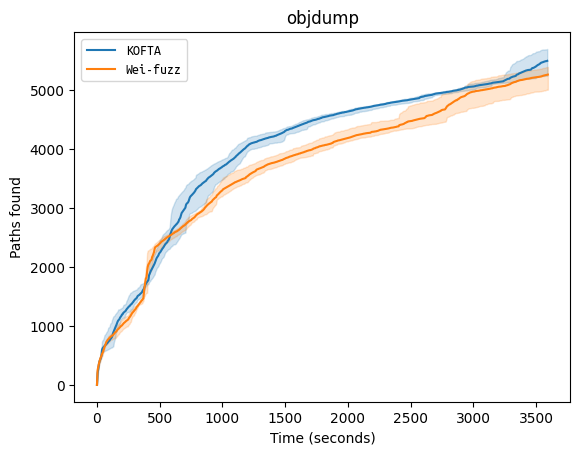
\includegraphics[width=0.8\textwidth]{img/1h/objdump-conf-1h.png}
    \end{subfigure}
    \begin{subfigure}[]{0.45\textwidth}
        \centering
        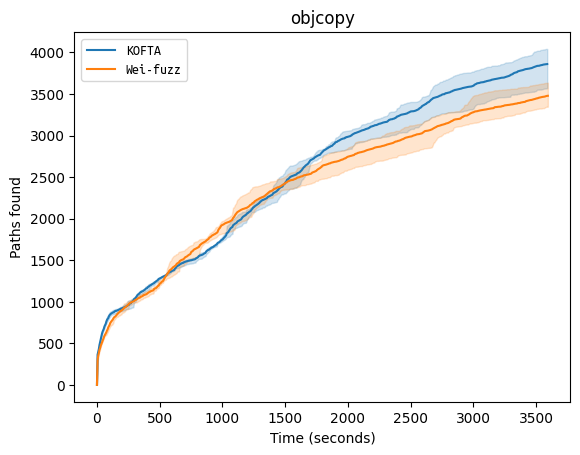
\includegraphics[width=0.8\textwidth]{img/1h/objcopy-conf-1h.png}
    \end{subfigure}
\end{figure}

\begin{figure}[h!]
    \centering
    \begin{subfigure}[]{0.45\textwidth}
        \centering
        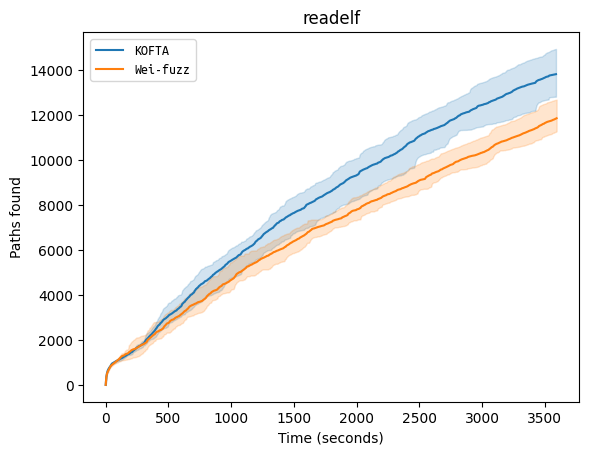
\includegraphics[width=0.8\textwidth]{img/1h/readelf-conf-1h.png}
    \end{subfigure}
    \begin{subfigure}[]{0.45\textwidth}
        \centering
        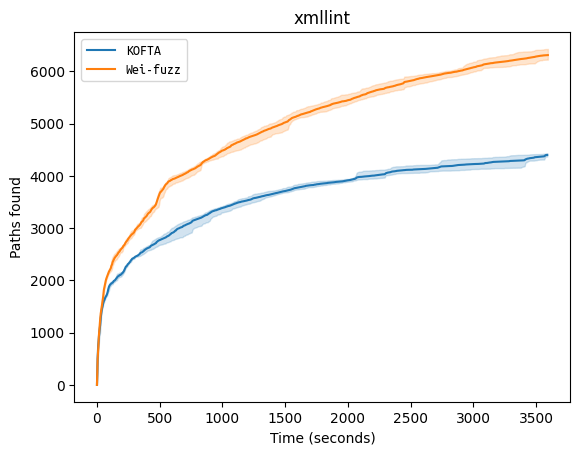
\includegraphics[width=0.8\textwidth]{img/1h/xmllint-conf-1h.png}
    \end{subfigure}
\end{figure}

\begin{figure}[h!]
    \centering
    \begin{subfigure}[]{0.45\textwidth}
        \centering
        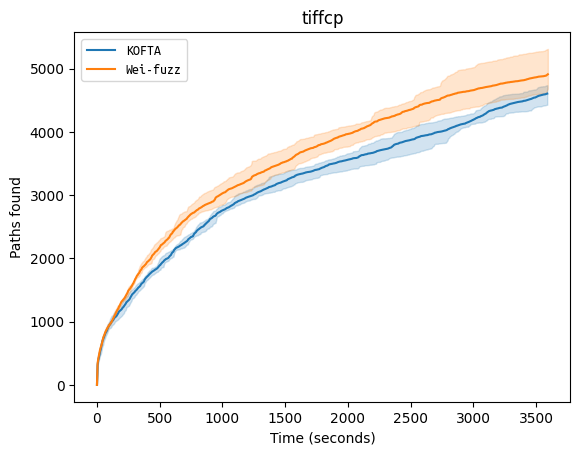
\includegraphics[width=0.8\textwidth]{img/1h/tiffcp-conf-1h.png}
    \end{subfigure}
    \begin{subfigure}[]{0.45\textwidth}
        \centering
        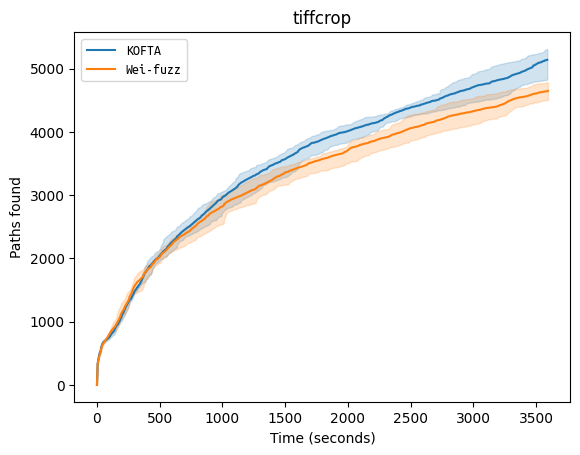
\includegraphics[width=0.8\textwidth]{img/1h/tiffcrop-conf-1h.png}
    \end{subfigure}
    \caption{KOFTA 選項參數 v.s. Wei-fuzz 選項參數}
    \label{fig:kofta-conf-vs-wei-conf}
\end{figure}


\iffalse
\begin{figure}[H] %[h!]
    \centering
    \begin{subfigure}[]{0.45\textwidth}
        \centering
        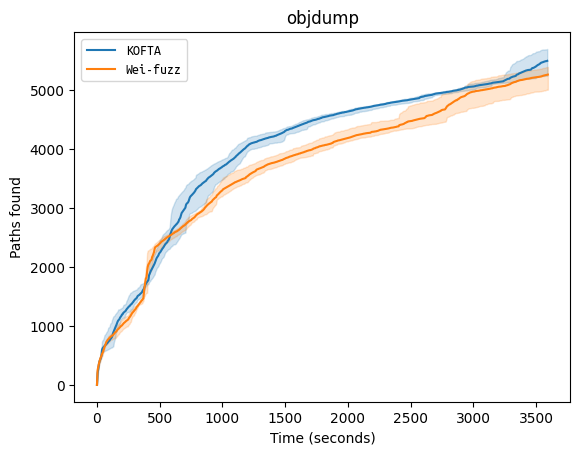
\includegraphics[width=0.8\textwidth]{img/1h/objdump-conf-1h.png}
    \end{subfigure}
    \begin{subfigure}[]{0.45\textwidth}
        \centering
        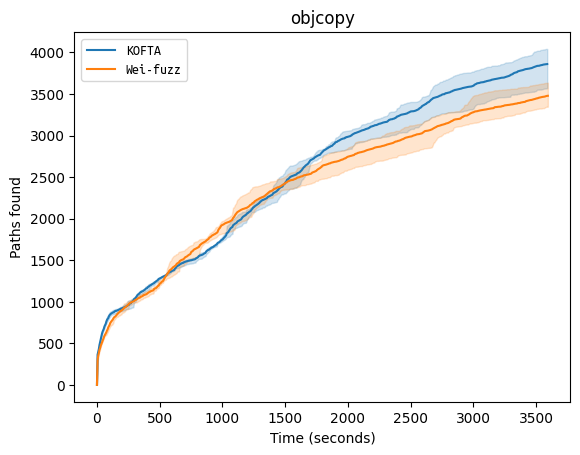
\includegraphics[width=0.8\textwidth]{img/1h/objcopy-conf-1h.png}
    \end{subfigure}
    \begin{subfigure}[]{0.45\textwidth}
        \centering
        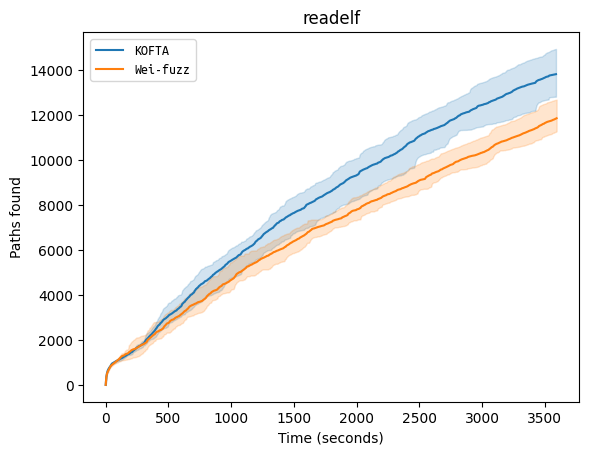
\includegraphics[width=0.8\textwidth]{img/1h/readelf-conf-1h.png}
    \end{subfigure}
    \begin{subfigure}[]{0.45\textwidth}
        \centering
        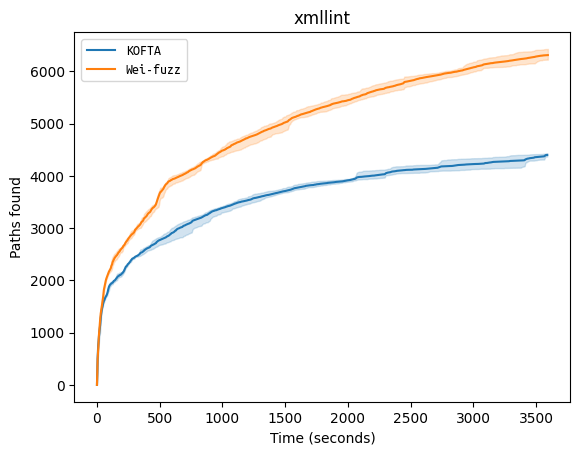
\includegraphics[width=0.8\textwidth]{img/1h/xmllint-conf-1h.png}
    \end{subfigure}
    \begin{subfigure}[]{0.45\textwidth}
        \centering
        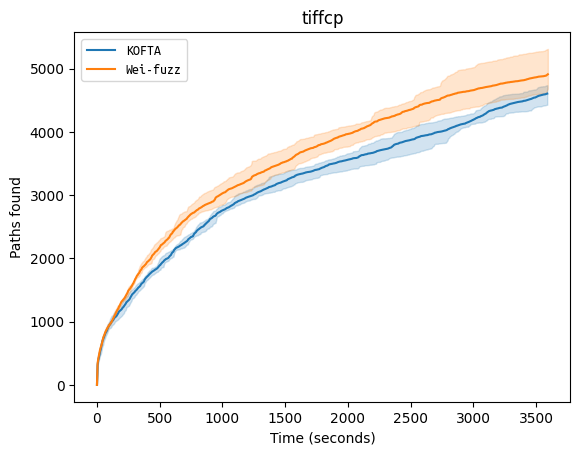
\includegraphics[width=0.8\textwidth]{img/1h/tiffcp-conf-1h.png}
    \end{subfigure}
    \begin{subfigure}[]{0.45\textwidth}
        \centering
        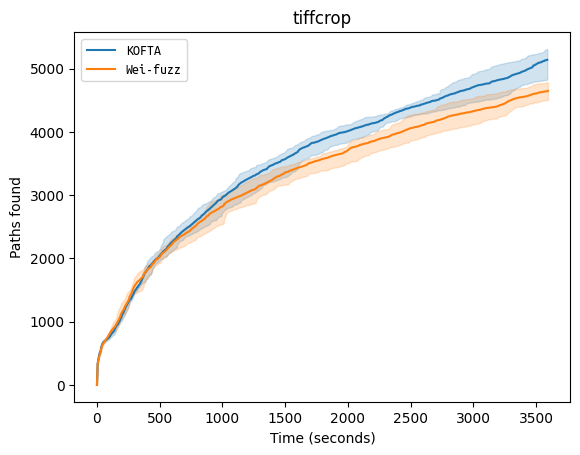
\includegraphics[width=0.8\textwidth]{img/1h/tiffcrop-conf-1h.png}
    \end{subfigure}
    \caption{KOFTA 選項參數 v.s. Wei-fuzz 選項參數}
    \label{fig:kofta-conf-vs-wei-conf}
\end{figure}
\fi

\fi % end of RQ3, RQ4
%\vfill\null

%\newpage

\subsection{RQ2}

%此實驗要探討的是「多參數 forkserver」實際帶來的影響。因為 KOFTA 使用「污染源推論」探索選項參數，需要比一般的多參數模糊測試工具更加頻繁地切換目標程式的命令列參數。比起 Wei-fuzz \cite{tseng2023wei}(在切換參數時需要重啟 forkserver），KOFTA 實作了可以直接更換命令列參數的 forkserver。為了驗證方法的有效性，我們提出了RQ:「多參數 forkserver 是否真的能夠減少多參數模糊測試的額外開銷？」。
This experiment explores the actual impact of a "multi-argument forkserver." Because KOFTA uses "taint inference" to explore option arguments, it requires switching the target program's command-line arguments more frequently than typical multi-argument fuzzing tools. Compared to Wei-fuzz (which requires restarting the forkserver when switching arguments), KOFTA implements a forkserver that allows direct switching of command-line arguments. %To verify the effectiveness of the method, we pose the question: "Does a multi-argument forkserver truly reduce the overhead of multi-parameter fuzzing?"

%在此實驗，以 KOFTA 與其變體 KOFTA-nf 進行測試比較 (KOFTA-nf：在切換命令列參數時會重啟 forkserver，如同 Wei-fuzz）。共有 10 個目標程式，實驗將測量 1 小時內目標程式的「執行次數」 (固定時間內的執行次數越高，代表額外開銷越低）。從結果（Table \ref{tab:kofta-vs-nf}）中可以看出，使用多參數 forkserver 的 KOFTA 有著更多的執行次數，代表污染源推論的額外開銷確實降低了；與 KOFTA-nf 相比，平均多出了約 44\% 的執行次數。
In this experiment, KOFTA and its variant KOFTA-nf were compared (KOFTA-nf restarts the forkserver when switching command-line parameters, similar to Wei-fuzz). Ten target programs were used, and the experiment measured the "execution counts" of each program within one hour (a higher number of executions within a fixed time indicates lower overhead). The results (Table \ref{tab:kofta-vs-nf}) show that KOFTA using the multi-argument forkserver has more executions, indicating a reduction in the overhead of taint inference; compared to KOFTA-nf, it has an average of approximately 44\% more executions.

\begin{table}[h!] %[hb]
    \centering
    \begin{threeparttable}
        \caption{\footnotesize Execution Counts (KOFTA v.s. KOFTA-nf)} %的執行次數
        \label{tab:kofta-vs-nf}
        \begin{tabularx}{0.5\textwidth}{
                >{\ttfamily}c|
                >{\ttfamily\centering\arraybackslash}X
                >{\ttfamily\centering\arraybackslash}X
                >{\ttfamily\centering\arraybackslash}X}
            \toprule
            \textbf{Program}  & \textbf{KOFTA\textsuperscript{*}} & \textbf{KOFTA-nf\textsuperscript{*}} & \textbf{\%} \\
            \midrule
            objdump        & ~8114943 & ~5411661 & ~+49.95\% \\
            objcopy        & ~9333905 & ~6802400 & ~+37.21\% \\
            readelf        & 11207506 & ~8027013 & ~+39.62\% \\
            xmllint        & ~8133153 & ~4645155 & ~+75.09\% \\
            tiffcp         & ~8456672 & ~7797795 & ~~+8.45\% \\
            tiffcrop       & ~9151116 & ~6675286 & ~+37.09\% \\
            mutool clean   & ~2690814 & ~2418753 & ~+11.25\% \\
            mutool convert & ~4580850 & ~2034483 & +125.16\% \\
            img2sixel      & ~7740032 & ~4806716 & ~+61.03\% \\
            giftool        & 19051953 & 12497357 & ~+52.45\% \\
            \midrule
            total          & 88460944 & 61116619 & ~+44.74\% \\
            \bottomrule
        \end{tabularx}
        \begin{tablenotes}
            \small
            \item \texttt{\textsuperscript{*}} = Total Execs
        \end{tablenotes}
    \end{threeparttable}
\end{table}

\iffalse
%產生額外開銷的不只污染源推論，文件變異階段也會。因此，這個實驗額外比較了 KOFTA-nd 與KOFTA-nfd 的執行次數 (變體 KOFTA-nd 是:跳過所有文件變異階段的 KOFTA；而變體 KOFTA-nfd 則是:不使用多參數 forkserver 版本的 KOFTA-nd）。測試時間同為 1 小時。因為沒有文件變異階段，所有的時間將投入污染源推論中，更能突顯污染源推論額外開銷的影響。如結果（Table \ref{tab:nd-vs-nfd}）所示，使用多參數 forkserver 的版本皆產生了更多的執行次數，在目標程式 \texttt{giftool} 的效果更是高達 347\%；平均而言，多出了約 256\%。與前述使用文件變異階段的 44\% 相比，這個結果突顯了多參數 forkserver 對於污染源推論的重要性。
The additional overhead isn't limited to taint inference; the file mutation phase also incurs it. Therefore, this experiment further compared the execution counts of KOFTA-nd and KOFTA-nfd (the KOFTA-nd variant skips all file mutation phases; the KOFTA-nfd variant does not use the multi-argument forkserver version of KOFTA-nd). The test duration was 1 hour for both. Because there's no file mutation phase, all time is devoted to taint inference, further highlighting the impact of its additional overhead. As shown in the results (Table \ref{tab:nd-vs-nfd}), KOFTA-nd consistently resulted in more executions, with a 347\% increase in the target program \texttt{giftool}; on average, an increase of approximately 256\%. Compared to the aforementioned 44\% increase using the file mutation phase, this result underscores the importance of the multi-argument forkserver for taint inference.

%\vfill

\begin{table}[h!] %[hb]
    \centering
    \begin{threeparttable}
        \caption{Execution Cnts (KOFTA-nd v.s. KOFTA-nfd)} %的執行次數
        \label{tab:nd-vs-nfd}
        \begin{tabularx}{0.5\textwidth}{
                >{\ttfamily}c|
                >{\ttfamily\centering\arraybackslash}X
                >{\ttfamily\centering\arraybackslash}X
                >{\ttfamily\centering\arraybackslash}X}
            \toprule
            \textbf{Program}  & \textbf{KOFTA\textsuperscript{*}} & \textbf{KOFTA-nf\textsuperscript{*}} & \textbf{\%} \\
            \midrule
            objdump        & 12539313 & ~2897087 & +332.82\% \\
            objcopy        & ~9193201 & ~2887072 & +218.43\% \\
            readelf        & 12458932 & ~3150788 & +295.42\% \\
            xmllint        & 12428781 & ~2821582 & +340.49\% \\
            tiffcp         & ~4156572 & ~2134392 & ~+94.74\% \\
            tiffcrop       & 10299351 & ~2461088 & +318.49\% \\
            mutool clean   & ~1314489 & ~1017056 & ~+29.24\% \\
            mutool convert & ~4422554 & ~2008962 & +120.14\% \\
            img2sixel      & ~~623140 & ~~566971 & ~~+9.91\% \\
            giftool        & 17729480 & ~3965936 & +347.04\% \\
            \midrule
            total          & 85165813 & 23910934 & +256.18\% \\
            \bottomrule
        \end{tabularx}
        \begin{tablenotes}
            \small
            \item \texttt{\textsuperscript{*}} = Total Execs
        \end{tablenotes}
    \end{threeparttable}
\end{table}
\fi